


\section{Method}



Given a real video and a semantic latent editing direction, we aim to produce an edited video. The outcome should preserve the fidelity of the original frames while modifying them in a temporally coherent manner, achieving meaningful and realistic editing.
To this purpose, we design a pipeline of six components: temporally consistent alignment, encoder-based inversion, generator tuning, editing, stitching tuning, and finally merging the results back into the original frame. In the following section, we describe in detail each core step, the tools used to implement it, and the motivation behind each choice. An overview of our full pipeline is presented in \cref{fig:pipeline}. In addition, a visualization of the state of the video at different stages of the editing pipeline is provided in \cref{fig:pipeline_example}.

\subsection{Alignment}\label{subsec:alignment} We employ a pre-trained StyleGAN2 model for face editing. This model, however, was trained on the FFHQ dataset, where each image was pre-processed. In particular, each image was cropped and aligned around the face. Inverting an image successfully into the latent space of the GAN thereby requires a similar crop-and-align phase. However, this pre-processing procedure consists of discrete steps (e.g. cropping) that are sensitive to the exact locations of extracted facial landmarks. This sensitivity can lead to the emergence of temporal inconsistencies, and thus we aim to reduce it. Inspired by the work of Fox et al.~\shortcite{fox2021stylevideogan}, we employ a gaussian lowpass filter over the landmarks. 
We find that this smoothing is sufficient to overcome any inconsistencies induced by the alignment step. 

\subsection{Inversion} To edit an aligned face, we must invert it into the latent space of the GAN. We do so using PTI \cite{roich2021pivotal}, a method which first discovers a 'pivot' latent code that approximately reconstructs the input image in the GAN's more editable regions, and then fine-tunes the \textit{generator} such that the same pivot code will produce a more accurate version of the target image. The goal of PTI was to overcome the distortion-editability trade-off \cite{tov2021designing} of inversion models, allowing for more accurate yet highly editable reconstructions. We argue that, beyond its original use, PTI can also assist in maintaining temporal coherency. The intuition here is that the original video which we wish to invert is itself temporally coherent. Therefore, if we can exactly reproduce each frame, we are guaranteed to have a coherent inversion.

In practice, however, we observe that PTI's editing performance is susceptible to inconsistencies in the pivots themselves. These manifest in two ways: First, if the pivots reside far from each other in the latent space, editing becomes less consistent. For example, the same face encoded in two different regions of the latent space might grow a different beard when the latent code is adjusted in the same direction. Second, if PTI has to 'fix' attributes (\eg a lack of beard) in the inversion, then further editing of the attribute will not typically account for this fix. As a consequence, if the attribute is inconsistent between pivots (a beard appearing in only some of the inverted frames), then PTI will only need to 'fix' it in some frames, and the resulting edit will differ around these frames.

We propose that both flaws can be corrected by simply replacing PTI's optimizer-based initial inversion (\ie finding the pivot) with an encoder-based version, and specifically e4e~\cite{tov2021designing}. As e4e is a deep neural network with many millions of parameters, it is inherently biased towards learning lower frequency representations~\cite{rahaman2019spectral}. We expect that this property will provide a strong smoothness bias, encouraging any coherent changes between images in consecutive frames to be mapped to coherently changing latent codes. In \cref{sec:quantitative}, we analyze this property and demonstrate that the use of an encoder does indeed outperform optimization-based inversions. Note that this property relies on the smoothness of transitions between input frames, and can hence be broken by inconsistent alignment, further motivating the changes of \cref{subsec:alignment}. To reduce memory and time requirements, we employ PTI around all pivot latent codes simultaneously (as opposed to a model for each frame).


Formally, given an $N$ frames source video $\{x_i\}^N_{i=1}$, we denote the cropped-and-aligned frames as $\{c_i\}^N_{i=1}$. We first use the e4e encoder $E$ to obtain their latent inversion $\{w_i\}^N_{i=1} = \{E(c_i)\}^N_{i=1}$. These latent vectors are then used as 'pivots' for PTI. Let $r_i = G(w_i; \theta)$ be the image generated from latent code $w_i$ with a generator $G$ parameterized by weights $\theta$, the PTI objective is defined as:
{\small
\begin{align}
\underset{\theta}{\min} \frac{1}{N}\sum^{N}_{i=1} ( \mathcal{L}_{\text{LPIPS}}(c_i, r_i) + \lambda^{\text{P}}_{L2}\mathcal{L}_{L2}(c_i, r_i)) + \lambda^{\text{P}}_R \mathcal{L}_{R}.
\end{align}
}
Where $\mathcal{L}_{\text{LPIPS}}$ is the LPIPS perceptual loss proposed by Zhang et al.~\shortcite{Zhang2018TheUE}, $\mathcal{L}_{L2}$ is pixel-wise MSE distance, and $\mathcal{L}_{R}$ is the locality regularization described by Roich et al.~\shortcite{roich2021pivotal}. $\lambda^{\text{P}}_{L2}, \lambda^{\text{P}}_R, $ are constants across all experiments.


\subsection{Editing}
Having acquired a set of temporally consistent inversions, we now turn to edit them. We demonstrate that our method works well with off-the-shelf linear editing techniques~\cite{shen2020interpreting,patashnik2021styleclip}.
We expect that, since StyleGAN itself is prone to low-frequency representations (and further motivated by path-length regularization), it will apply sufficiently consistent edits for nearby latent codes. In other words, if we edit temporally-smooth pivots using StyleGAN, we expect to generate a temporally smooth sequence. As we later demonstrate, this expectation aligns with our experimental results. Formally, given a semantic latent editing direction $\delta w$, we utilize the PTI-weights $\theta_p$ to obtain our edited frames $e_i = G(w_i+\delta w; \theta_p)$. 

\subsection{Stitching Tuning}

\vspace{-0.1cm}
\begin{figure}[tb]
    \centering
    \setlength{\belowcaptionskip}{-5pt}
    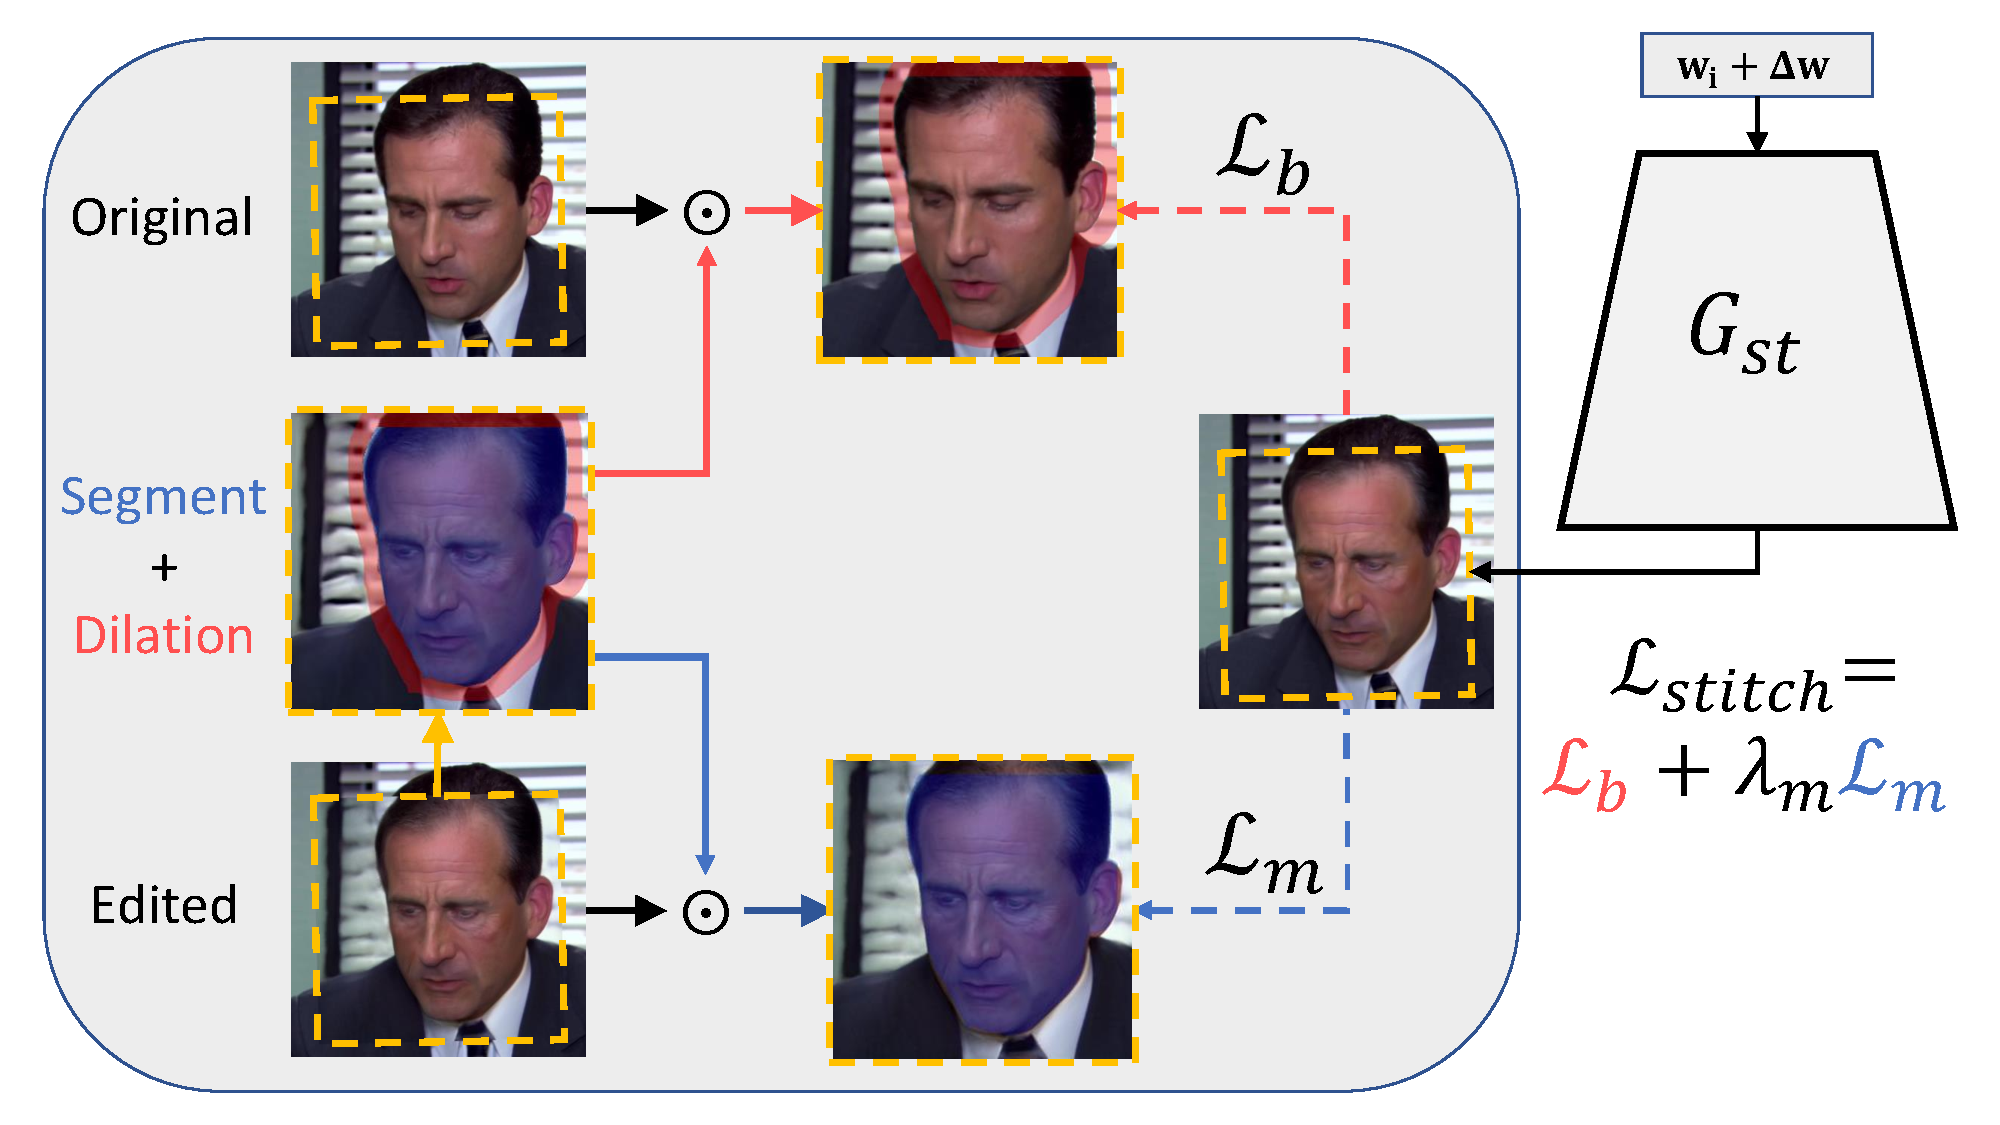
\includegraphics[width=0.99\linewidth]{resources/images/stitching.pdf}
    % \vspace{-0.25cm}
    \caption{
    Outline of our stitching-tuning method. We start with generating an edited image using a modified pivot code and segment the image using an off-the-shelf segmentation network \cite{yu2021bisenet}. The segmentation mask is dilated, creating a boundary region. We then fine-tune the generator so that the modified pivot will provide an image that is $(a)$ consistent with the original edit inside the face mask (blue), and $(b)$ consistent with the original background inside the boundary mask (red). We synthesize the final image using the tuned generator and paste it inside the dilated mask region (blue + red).
    }
    % \vspace{-0.2cm}
    \label{fig:stitching}
\end{figure}

As a final step, we must inject the edited face $e_i$ back into the original video. Merely overwriting the original location of the cropped face is insufficient, as the editing process typically leads to changes in the background which are noticeable around the crop boundary. For instance, \cref{fig:pipeline_example,fig:ablation} demonstrate that artifacts emerge when stitching the crop {\naive}ly. Prior works~\cite{yao2021latent} elected to limit the modifications to the face area by using segmentation masks derived from the landmarks detected in the alignment step and performing Poisson blending. Such stitching, however, is still prone to inconsistencies around the border, leading to artifacts such as the appearance of ghostly outlines (see \cref{fig:comparison}). We propose to tackle this limitation through a novel tuning technique inspired by PTI, referred to as \textit{stitching tuning}. An overview of this technique is provided in \cref{fig:stitching}. For each edited frame, we designate a boundary at the edge of the segmentation mask. We then briefly fine-tune our generator around the \textit{edited pivot} with a dual objective. First, we aim to restore the boundary to its pre-inversion values, that is to blend it perfectly in the original frame. Second, we wish to retain our editing results, by requiring similarity to the edited frame in the area covered by the segmentation mask. This short tuning session can successfully restore the boundary and induce a smooth transition towards the center of the image, without affecting the edited face. 

Formally, we first use off-the-shelf pre-trained segmentation network \cite{yu2021bisenet} to produce segmentation masks $\{m_i\}^N_{i=1}$ for all frames. We then perform dilation on each to obtain a set of expand masks $\{m^d_i\}^N_{i=1}$. The boundary is defined as their element-wise \textit{xor} operator $\{b_i\}^N_{i=1} = \{m_i \oplus m^d_i\}^N_{i=1}$. Let $s_i = G(w_i+\delta w; \theta_{st})$ denote the outcome of the stitching tuning procedure, our first objective is blending the boundary to the original image:
\begin{align}
\mathcal{L}_{b,i} = \mathcal{L}_{L1}(s_i \odot b_i, x_i \odot b_i),
\end{align}
where $\odot$ is the element-wise multiplication. The second objective is preserving the editing result:
\begin{align}
\mathcal{L}_{m,i} = \mathcal{L}_{L1}(s_i \odot m_i, e_i \odot m_i).
\end{align}
These loss terms used to further optimize the generator weights $\theta_{st}$ for each frame:
\begin{align}
\underset{\theta_{st}}{\min} \mathcal{L}_{b,i} + \lambda_m\mathcal{L}_{m,i} , 
\end{align}
where the weights are initialized with the PTI weights $\theta_p$, and  $\lambda_m$ is constant across all experiments. Finally, we perform the inverted alignment and stitch each frame $s_i$ to the original frame $x_i$ using the dilated masks $\{m^d_i\}^N_{i=1}$. Gaussian blur might be applied to further smooth the edges of the masks.


\subsection{Implementation Details}

For all experiments, we set $\lambda^{\text{P}}_{L2} = 10$, $\lambda^{\text{P}}_R = 0.1 $ and $\lambda_m = 0.01$. When tuning a model with PTI we use a learning rate of $3e-5$ and train until each frame is observed 80 times. When tuning a model for stitching, we increase the learning rate to $3e-4$ and the number of training iterations to 100 per frame. For all other implementation details we follow PTI.

% This allows us to reduce editing times from approximately 5 hours per video to approximately 50 minutes on a single NVIDIA 2080 RTX. \rmc{The real reason is that it actually produce an even smoother result. Rinon, Let's add it to the main text}



